\documentclass[12pt,fleqn]{article}\usepackage{../../common}
\begin{document}
Sinyaller, Geriye Dönük Analiz, Performans

Elimizde bir zaman serisi var, bu seri bir finansal varlığın fiyat seviyesi
olabilir, belki Apple senedidir, ilk gün 100 ikinci gün 102 olmuş, böyle
gidiyor.

\begin{minted}[fontsize=\footnotesize]{python}
import pandas as pd
d = np.array([100,102,104.04,106.12,108.24,110.41])
\end{minted}

Peki bu fiyat seviyeleri günlük hangi yüzde değişimlerine tekabül ediyor?
Bu hesabın bir yolu var, \verb!pct_change! kullanabiliriz,

\begin{minted}[fontsize=\footnotesize]{python}
p = pd.Series(d)
print (list(p))
print (list(np.round(p.pct_change(),2)))
\end{minted}

\begin{verbatim}
[100.0, 102.0, 104.04, 106.12, 108.24, 110.41]
[nan, 0.02, 0.02, 0.02, 0.02, 0.02]
\end{verbatim}

Her gün yüzde 2'lik bir değişim varmış (bu yazı için veri uydururken sayıları
ona göre ayarladık).

Şimdi sadece yüzde değişimleri ve başlangıç fiyat seviyesini kullanarak seriyi
tekrar üretebilir miydik? Tek yüzde değişimle bir sonraki sayıyı nasıl elde
ederiz?  Mesela 100'den yüzde 2 değişimle sonraki değere geçeceğiz, kolay, 1
artı 0.02 yani 1.02 değerini 100 ile çarparız, sonraki sayı çıkar, 102. Bu
metotu diğer yüzde değişimler için kullanabiliriz. O zaman tüm fiyat
seviyelerini hesap için eldeki yüzde değişim listesine 1 sayısını eklersek,
1.02, 1.02, .. elde edilir, ve bu rakamları başta 100 ile, sonra birbirleri ile
çarparsak tüm fiyat listesini tekrar elde ederiz. Bir dizinin tüm öğelerinin
birer birer çarpılıp bunun kümülatif olarak gösterilmesini \verb!cumprod!
halleder,

\begin{minted}[fontsize=\footnotesize]{python}
ret = p.pct_change()
100*np.cumprod(1+ret)
\end{minted}

\begin{verbatim}
Out[1]: 
0       NaN
1    102.00
2    104.04
3    106.12
4    108.24
5    110.41
dtype: float64
\end{verbatim}

Üstteki hesabı bir al-tut stratejisinin performansı olarak ta görebiliriz bu
durumda illa baştaki 100 değerini kullanmaya gerek yok, 100 yerine 1 dersek o
zaman bu stratejiye koyulmuş 1 liranın, 1 doların ne kadar büyüyeceğini görmüş
oluruz.  1 lira 2 lira olduysa mesela bu ikiye katlama demektir, performansın
iyi olduğu sonucuna varabiliriz.

\begin{minted}[fontsize=\footnotesize]{python}
1*np.cumprod(1+ret)
\end{minted}

\begin{verbatim}
Out[1]: 
0       NaN
1    1.0200
2    1.0404
3    1.0612
4    1.0824
5    1.1041
dtype: float64
\end{verbatim}

Yüzde değişimler, kumulatif çarpımlar ile uğraşmamızın bir sebebi var, portföy
perfomansına bakarken herhangi bir strateji için gereken alım / satım
``sinyallerini'' kolayca dahil edebiliyoruz, ve stratejiyi tartarken bir zaman
serisi üzerinden bunu yapabiliyoruz. Elde edilecek serinin istatistiki,
matematiksel özellikleri vardır, ve bu özellikleri ek özet irdelemeler
faydalı olur, mesela Sharpe oranı gibi.

Sinyalleri şöyle kullanabiliriz, bir varlığı belli bir zaman noktasında almış
olmak 1 sinyali ile temsil edilir, varlığın elde olmaması ise 0 ile temsil
edilir.  O zaman kumulatif hesaptan önce tüm yüzde değişimleri sinyal vektörü
ile çarparız, ondan sonra kumulatif hesap devreye girer. Eğer sinyal 1 ise o
noktada yüzde değişim sıfıra iner, o getiri elde edilmemiş olur, kumulatif
hesapta 1+0 = 1, yani hiç bir değişim yaratmaz. Eğer sinyal 1 ise 1 çarpı mesela
yüzde 2 getiri yüzde 2 getirinin aktif olmuş olması demektir, o getiri kumulatif
çarpıma etki eder.

\begin{minted}[fontsize=\footnotesize]{python}
signal = pd.Series(np.array([1,1,1,1,0,1]))
ret*signal
\end{minted}

\begin{verbatim}
Out[1]: 
0         NaN
1    0.020000
2    0.020000
3    0.019992
4    0.000000
5    0.020048
dtype: float64
\end{verbatim}

\begin{minted}[fontsize=\footnotesize]{python}
signal = pd.Series(np.array([1,1,1,1,0,1]))
1*np.cumprod(1+(ret*signal))
\end{minted}

\begin{verbatim}
Out[1]: 
0         NaN
1    1.020000
2    1.040400
3    1.061200
4    1.061200
5    1.082475
dtype: float64
\end{verbatim}

Senet Ornegi

Apple senedine bakalim,

\begin{minted}[fontsize=\footnotesize]{python}
import pandas as pd
df = pd.read_csv('../tser_008_data/AAPL.csv',index_col='Date',parse_dates=True)
df.plot()
plt.savefig('tser_011_sign_01.jpg')
\end{minted}

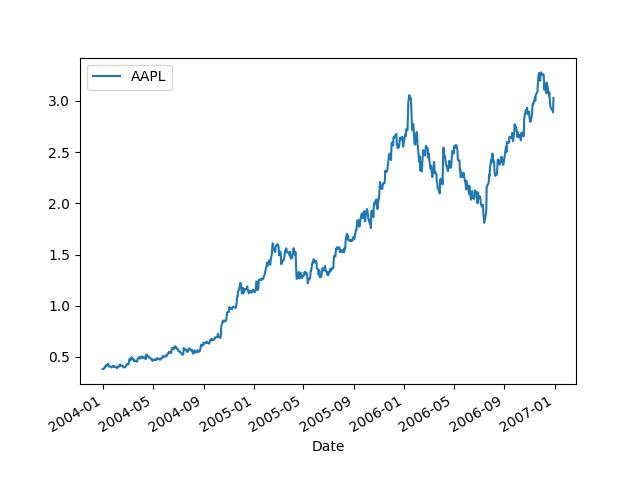
\includegraphics[width=20em]{tser_011_sign_01.jpg}

\begin{minted}[fontsize=\footnotesize]{python}
df['signal'] = 0
filt1 = (df.index > '2005-06-01') & (df.index < '2006-02-01')
df.loc[filt1,'signal'] = 1
filt2 = (df.index > '2006-09-01') & (df.index < '2007-01-01')
df.loc[filt2,'signal'] = 1
df['ret'] = df.AAPL.pct_change()

cumret = np.cumprod(1+(df.ret*df.signal))
print (cumret.tail(4))
\end{minted}

\begin{verbatim}
Date
2006-12-26    2.233475
2006-12-27    2.233750
2006-12-28    2.215938
2006-12-29    2.324721
dtype: float64
\end{verbatim}


\begin{minted}[fontsize=\footnotesize]{python}
np.prod(1+(df.ret*df.signal))
\end{minted}

\begin{verbatim}
Out[1]: 2.3247214450625857
\end{verbatim}

\begin{minted}[fontsize=\footnotesize]{python}
print ('APR', ((np.prod(1.+df.ret*df.signal))**(252./len(df.ret)))-1)
\end{minted}

\begin{verbatim}
APR 0.32471861974412564
\end{verbatim}

\begin{minted}[fontsize=\footnotesize]{python}
df = pd.read_csv('../tser_008_data/AAPL.csv',index_col='Date',parse_dates=True)
df['signal'] = 0
filt1 = (df.index > '2005-06-01')
df.loc[filt1,'signal'] = 1
df['ret'] = df.AAPL.pct_change()
print (np.prod(1+(df.ret*df.signal)))
print ('APR', ((np.prod(1.+df.ret*df.signal))**(252./len(df.ret)))-1)
\end{minted}

\begin{verbatim}
2.105210500206348
APR 0.2816374105511763
\end{verbatim}


















[devam edecek]
  
\end{document}
